% ======================================================================
\section{Numerical Experiments}\label{sec:numerics}

\subsection{Setup}\label{subsec:protocol}
Each subsection names the MATLAB test file that produces its results. The accuracy tests at moderate size
use leaves of 16--64 rows, so that every tree has 3--7 levels; the timing and large-$n$ runs use leaves of
200--400 rows. \PlatformSentence

With $x$ the computed solution, we report:
\begin{itemize}[leftmargin=1.5em,itemsep=1pt]
\item the residual $\|Hx-b\|/\|b\|$;
\item the \emph{solver error} $\|x-x_{\rm ref}\|/\|x_{\rm ref}\|$, where $x_{\rm ref}$ is the dense minimum-norm
solution of the HSS matrix itself, computed from a QR factorization $H^*=QR$ as $x_{\rm ref}=Q(R^{-*}b)$. This
measures the solver alone, without the compression error;
\item the error against the minimum-norm solution of the original matrix $A$, which adds the compression
error;
\item the null-space fraction $\|P_{\mathcal N(H)}x\|/\|x\|$, which is $0$ for an exact minimum-norm solution;
\item for large $n$, where no dense matrix can be formed, the error against a \emph{manufactured}
solution: draw $z$, set $x_\star=H^*z$ and $b=Hx_\star$. Since $x_\star\in\operatorname{Range}(H^*)$ and
$Hx_\star=b$, $x_\star$ \emph{is} $H^+b$, and $\|x-x_\star\|/\|x_\star\|$ needs only HSS products.
\end{itemize}

\subsection{Test matrices}\label{subsec:testmatrices}
Table~\ref{tab:families} defines the families. F1 and F2 are given directly by their generators, so they
are exactly HSS; F3--F6 are compressed from their entries with nested interpolative decompositions.
Large-$n$ cases never form a dense matrix.

\begin{table}[!htb]
\centering\footnotesize
\setlength{\tabcolsep}{4pt}
\begin{tabular}{@{}l>{\raggedright\arraybackslash}p{8.4cm}>{\raggedright\arraybackslash}p{3.3cm}>{\raggedright\arraybackslash}p{1.9cm}@{}}
\toprule
& definition & HSS form & $\kappa$\\
\midrule
F1 & $A=XY+\operatorname{blkdiag}(E_\tau)$, $X\in\mathbb{R}^{m\times k}$, $Y\in\mathbb{R}^{k\times n}$, $E_\tau\in\mathbb{R}^{n_\tau\times p_\tau}$ (one block per leaf), entries iid $U[0,1]$ & exact, rank $k$ ($U_\tau=X(I_\tau,:)$, $V_\tau=Y(:,J_\tau)^T$, $R=W=[I;I]$, $B=I$) & \KFone, grows $\propto n$\\
F2 & random HSS: $D_\tau$ iid $N(0,1)/\sqrt{p_\tau}$; $U,V,R,W$ with orthonormal columns (QR of Gaussian matrices); $B$ iid $N(0,1)/\sqrt k$; real or complex & exact, rank $k$ & \KFtwo\\
F2$_\alpha$ & F2 with graded columns: $H\operatorname{diag}(10^{-\alpha u_j})$, $u_j$ iid $U[0,1]$, $\alpha\ge0$ & exact, same ranks as F2 & \KFtwoG\\
F3 & $A_{ij}=1/(x_i-y_j)$, $x_i=i$ ($i\le M$), three points $y=x_i+q/4$ ($q=1,2,3$) in each gap; $n=3(M-1)$ & tolerance $10^{-10}$ & \KFthree\\
F4 & $y_i=\sum_jg(si+w-j)\,x_j$: Gaussian (width $\sigma$) or Ricker wavelet $g$, truncated at $|d|\le w=\lceil4\sigma\rceil$; stride $s$; ``valid'' outputs only & exact (banded) & \KFfour, grows with $\sigma$\\
F5 & $C=AF^*$ with $A_{jk}=e^{2\pi ikx_j}$, $k=-N/2,\dots,N/2-1$, jittered $x_j$, $F$ the unitary DFT: $C_{jl}=D_N(x_j-l/N)/\sqrt N$, $D_N$ the Dirichlet kernel; complex & tolerance $10^{-12}$ & \KFfive\\
F6 & $C=F_mTD^*F_n^*$ with $T\in\mathbb{R}^{m\times 2m}$ random Toeplitz, $F_m,F_n$ unitary DFTs, $D$ a unit-modulus diagonal & tolerance $10^{-12}$ & \KFsix\\
\bottomrule
\end{tabular}
\caption{Test families. All are wide ($m<n$) and of full row rank. $\kappa$ at the sizes of Table~\ref{tab:e1}
(F2$_\alpha$ and F4: over the sweeps of Section~\ref{subsec:stab}).}
\label{tab:families}
\end{table}

\paragraph{Notes on the families.}
F1 has a rank-$k$ part with all-positive entries. Its largest singular value is therefore about
$\tfrac k4\sqrt{mn}$, far above the rest of the spectrum, so $\kappa(\mathrm{F1})$ grows linearly with $n$,
and so does the error at large $n$ (Section~\ref{subsec:large}). F2 is the generic case: fixed rank and
a small condition number. Scaling its columns (F2$_\alpha$) keeps it exactly HSS with the same ranks and raises
$\kappa$ steadily with $\alpha$ (roughly like $10^{\alpha/2}$), which makes $\kappa$ a parameter. F3 is a smooth kernel matrix;
interlacing the two point sets keeps $\kappa\approx2$ at every size. F4 is a decimated convolution, as in
deconvolution with a ``valid'' boundary or a stride: it is banded and therefore exactly HSS, and its
condition number is set by the blur width $\sigma$. We use it to compare the direct solver with
iterative methods as $\kappa$ grows (Section~\ref{subsec:stab}). F5 and F6 come from matrices that are not
HSS themselves: a nonuniform Fourier matrix, as in interpolating a band-limited signal from irregular
samples, and a random Toeplitz matrix, whose off-diagonal blocks have full rank. Unitary DFTs turn both
into Cauchy-like matrices, which are HSS~\cite{gko}. By Lemma~\ref{lem:twosided}, a unitary change of
variables maps minimum-norm solutions to minimum-norm solutions, so the solver applies to the transformed
system unchanged.

\subsection{Correctness at moderate size}\label{subsec:correct}
Table~\ref{tab:e1} runs every family at a size where the dense references are affordable
(\texttt{mp\_exp\_correctness.m}). In every case the residual is at most $\EoneMaxRes$ and the solver error is at most
$\EoneMaxErrOverKappaU\,\kappa(H)u$\EoneSmallKappaClause. The null-space fraction, the part of $x$ that a minimum-norm solution
must not have, is of the same size as the solver error; a method that solved $Hx=b$ but drifted from the
minimum-norm solution would show a null-space fraction far above the residual. The error against the
original matrix adds the compression error: for F3, F5 and F6 it is $\EoneCompMin$--$\EoneCompMax$, of
the size of the compression tolerance ($10^{-10}$ for F3, $10^{-12}$ for F5 and F6), as the
$2\kappa\varepsilon$ bound of Section~\ref{sec:proof} predicts; for F1, F2 and F4, which are exactly HSS, it
agrees with the solver error.
The cases \EoneNoSlack{} violate the slack condition of Assumption~\ref{as:slack} and are as accurate as
the others.

\begin{table}[!htb]
\centering\scriptsize
\setlength{\tabcolsep}{3pt}
\begin{tabular}{@{}lrrrrrcccccc@{}}
\toprule
case & $m$ & $n$ & $L$ & rank & $\kappa(H)$ & As.~\ref{as:slack} & residual & solver error & null frac. & vs.\ $A$\\
\midrule
F1 & 320 & 480 & 4 & 3 & $1.3{\times}10^{3}$ & yes & $5.9{\times}10^{-15}$ & $2.3{\times}10^{-14}$ & $1.6{\times}10^{-14}$ & $2.3{\times}10^{-14}$\\
F1 & 2048 & 4096 & 7 & 3 & $7.4{\times}10^{3}$ & yes & $2.8{\times}10^{-14}$ & $1.9{\times}10^{-13}$ & $1.7{\times}10^{-13}$ & $1.9{\times}10^{-13}$\\
F2 & 1024 & 2048 & 5 & 10 & 14 & yes & $1.4{\times}10^{-15}$ & $3.6{\times}10^{-15}$ & $3.2{\times}10^{-15}$ & $3.6{\times}10^{-15}$\\
F2 complex & 1024 & 2048 & 5 & 10 & 13 & yes & $1.5{\times}10^{-15}$ & $5.2{\times}10^{-15}$ & $4.6{\times}10^{-15}$ & $5.2{\times}10^{-15}$\\
F2 $m/n=0.9$ & 1800 & 2000 & 5 & 8 & 79 & no & $2.5{\times}10^{-15}$ & $1.4{\times}10^{-14}$ & $1.2{\times}10^{-14}$ & $1.4{\times}10^{-14}$\\
F3 & 1024 & 3069 & 5 & 32 & 1.9 & yes & $1.1{\times}10^{-15}$ & $2.2{\times}10^{-15}$ & $2.2{\times}10^{-15}$ & $6.7{\times}10^{-11}$\\
F4 Gaussian, $\sigma=2$, $s=2$ & 2040 & 4096 & 5 & 10 & 98 & yes & $6.6{\times}10^{-15}$ & $1.0{\times}10^{-14}$ & $8.7{\times}10^{-15}$ & $1.0{\times}10^{-14}$\\
F4 Ricker, $\sigma=3$, $s=2$ & 2036 & 4096 & 5 & 15 & $2.2{\times}10^{3}$ & yes & $7.7{\times}10^{-14}$ & $1.9{\times}10^{-13}$ & $1.9{\times}10^{-13}$ & $2.0{\times}10^{-13}$\\
F4 Gaussian, $\sigma=3$, $s=3$ & 1358 & 4096 & 5 & 10 & 98 & yes & $5.1{\times}10^{-15}$ & $1.0{\times}10^{-14}$ & $9.3{\times}10^{-15}$ & $1.0{\times}10^{-14}$\\
F5 & 1536 & 2048 & 5 & 36 & 2.0 & no & $1.2{\times}10^{-15}$ & $3.1{\times}10^{-15}$ & $3.1{\times}10^{-15}$ & $1.0{\times}10^{-12}$\\
F6 & 1024 & 2048 & 5 & 62 & 7.4 & no & $2.1{\times}10^{-15}$ & $4.2{\times}10^{-15}$ & $3.7{\times}10^{-15}$ & $1.4{\times}10^{-12}$\\
\bottomrule
\end{tabular}

\caption{Accuracy at moderate size. ``rank'': largest generator rank; $L$: depth; ``As.~\ref{as:slack}'':
whether every leaf satisfies the slack condition. ``vs.\ $A$'': error against the minimum-norm solution
of the original matrix (for F6, in the Toeplitz variables, $x=D^*F_n^*y$).}
\label{tab:e1}
\end{table}

\subsection{Accuracy as the condition number grows}\label{subsec:stab}
Figure~\ref{fig:stab} sweeps $\kappa(H)$ in the two families where it is a parameter, F2$_\alpha$ (depth 3)
and F4 with stride 1 and growing $\sigma$ (depth 4), and compares the ULV solve with the normal equations
(Cholesky factorization of $HH^*$) and with CGNE (conjugate gradients on $HH^*$ with HSS products,
relative-residual tolerance $10^{-14}$, at most 2000 iterations). All are measured against the dense QR
solution (\texttt{mp\_exp\_conditioning.m}). For an ill-conditioned problem that reference is itself
accurate only to about $\kappa u$ ($u\approx1.1\times10^{-16}$), so differences below $\kappa u$ cannot be
resolved: a curve at or below the $\kappa u$ line means the method is as accurate as dense QR.

The ULV solution stays within $\EtwoUlvOverKappaU\,\kappa u$ of the dense QR solution over the whole range,
up to $\kappa\approx\EtwoMaxKappaGraded$ for F2$_\alpha$ and $\EtwoMaxKappaBlur$ for F4: it is as accurate as
dense QR. The normal equations follow $\kappa^2u$, as squaring the condition number predicts, and their
Cholesky factorization fails from $\kappa\approx\EtwoCholFailGraded$ (F2$_\alpha$) and $\EtwoCholFailBlur$ (F4) on.
CGNE needs $\EtwoCgItsMinGraded$ iterations already at $\kappa\approx10$; from $\kappa\approx\EtwoCgFailGraded$
(F2$_\alpha$) and $\EtwoCgFailBlur$ (F4) on it does not converge within 2000 iterations and its error exceeds
$10^{-6}$. This is the regime that needs a direct solver. The backward error
$\|b-Hx\|/(\|H\|\|x\|+\|b\|)$, which needs no reference, is the smallest relative perturbation of $H$ and
$b$ for which $x$ solves the system exactly; it stays below $\EtwoUlvBwdMax$ for the ULV solution throughout
(dense QR: $\EtwoQrBwdMax$) and grows to $\EtwoNeBwdMax$ for the normal equations.

\begin{figure}[!htb]
\centering
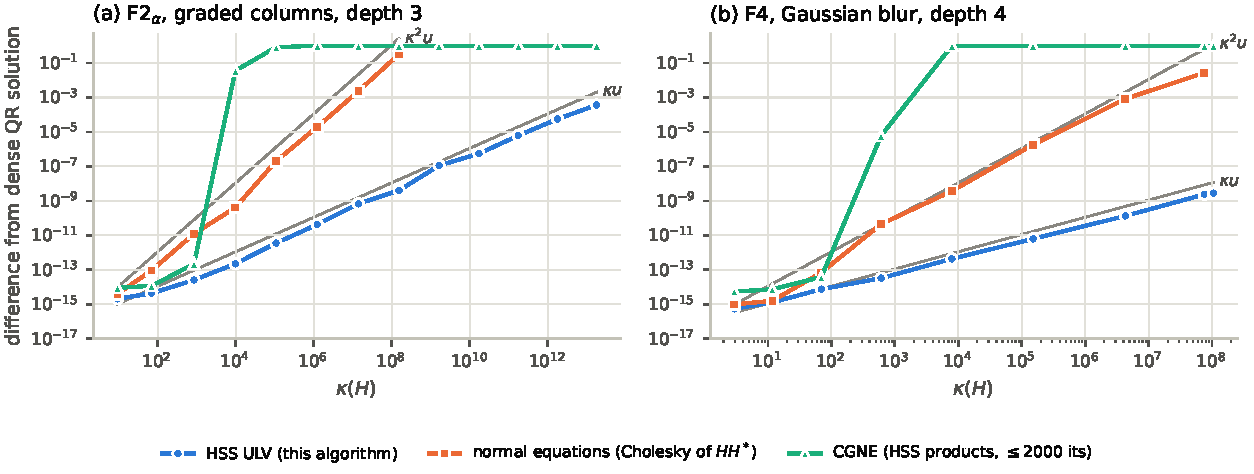
\includegraphics[width=\textwidth]{figures/m1_stability.pdf}
\caption{Relative difference from the dense QR minimum-norm solution as $\kappa(H)$ grows. (a) F2$_\alpha$,
$128\times256$, depth 3; (b) F4, Gaussian blur, stride 1, $\approx290\times300$, depth 4. Grey lines:
$\kappa u$ and $\kappa^2u$. Missing normal-equation points: the Cholesky factorization of $HH^*$ failed.
CGNE values of 1: no iterate had a smaller residual than the starting guess $0$, which is returned.}
\label{fig:stab}
\end{figure}

\subsection{Accuracy at large $n$}\label{subsec:large}
With manufactured solutions the solver can be checked at sizes where no dense matrix fits
(Figure~\ref{fig:largescale}, \texttt{mp\_exp\_scaling.m}, the same run as Figure~\ref{fig:complexity}).
For F2--F5 the error stays between $\EthreeErrMin$ and $\EthreeErrMax$ for every $n$ up to $\EfourMaxN$.
For F1 it grows from $\EthreeFoneFirst$ to $\EthreeFoneLast$, in step with $\kappa(\mathrm{F1})\propto n$
(Section~\ref{subsec:testmatrices}): this is the conditioning of the test matrix, not error growth in the
solver. Residuals are at most $\EthreeMaxRes$.

\begin{figure}[!htb]
\centering
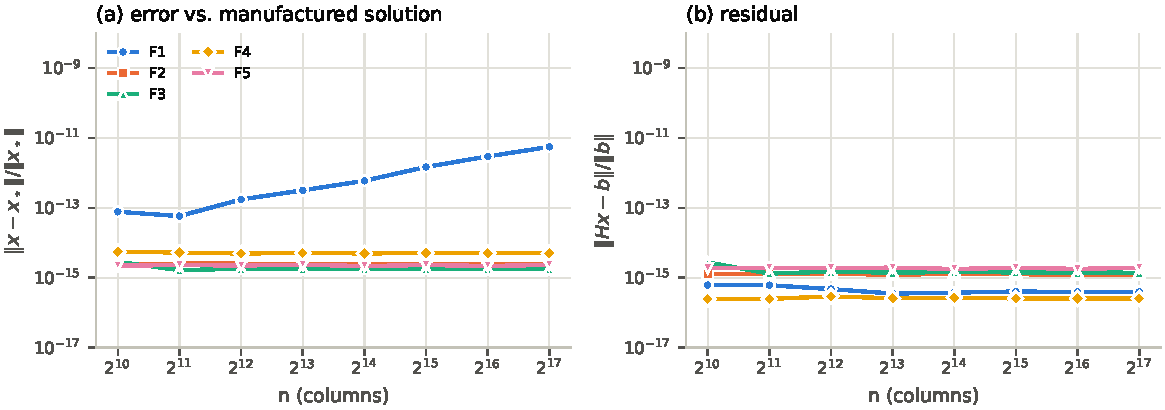
\includegraphics[width=0.92\textwidth]{figures/m1_largescale_accuracy.pdf}
\caption{Error against the manufactured minimum-norm solution as $n$ grows. No dense matrix is formed.}
\label{fig:largescale}
\end{figure}
